\documentclass[a4paper,12pt]{article}

\usepackage{mystyle}
\usepackage{gensymb}


\usepackage{scalerel}
\usepackage{stackengine}

\graphicspath{ {images/} }


\definecolor{violet}{RGB}{148, 0, 211}
\definecolor{red}{RGB}{183, 65, 14}
\definecolor{cyan}{RGB}{0, 166, 147}


% https://tex.stackexchange.com/a/101138/135045

\newcommand\widesim[1]{\ThisStyle{%
  \setbox0=\hbox{$\SavedStyle#1$}%
  \stackengine{-.1\LMpt}{$\SavedStyle#1$}{%
    \stretchto{\scaleto{\SavedStyle\mkern.2mu\sim}{.5150\wd0}}{.6\ht0}%
  }{O}{c}{F}{T}{S}%
}}

\newcommand{\BigMiddleTwo}{\;\left|\vphantom{\begin{pmatrix} 0\\0 \end{pmatrix}}\right.\;}
\newcommand{\BigMiddleThree}{\;\left|\vphantom{\begin{pmatrix} 0\\0\\0 \end{pmatrix}}\right.\;}



% https://tex.stackexchange.com/questions/9641/filled-diamondsuit-and-heartsuit
\DeclareSymbolFont{extraup}{U}{zavm}{m}{n}
\DeclareMathSymbol{\varheartsuit}{\mathalpha}{extraup}{86}
\DeclareMathSymbol{\vardiamond}{\mathalpha}{extraup}{87}


% https://tex.stackexchange.com/questions/234942/whats-the-best-way-to-make-a-heart-butt-in-latex
\newcommand{\heart}{\ensuremath\varheartsuit}




\author{Алексеев Василий}


\title{Семинар 2}
\date{10 + 14 февраля ($\heart$) 2022}


\begin{document}
  \maketitle
  
  \tableofcontents

  \thispagestyle{empty}
  
  \newpage
  
  \pagenumbering{arabic}


  \section{Системы линейных уравнений}
  
  \paragraph{Пример на пальцах номер $1$.}
  
  Рассмотрим систему:
  \[
    \left\{ \begin{aligned}
      &x + y = 1\\
      &x - y = 1
    \end{aligned} \right.
  \]
  
  Два уравнения, две неизвестных.
  Как можно решить систему?
  Её можно решить методом Крамера (см. первый семинар прошлого семестра).
  Или подстановкой (выразить из одного уравнения одну переменную через другую, подставить в оставшееся уравнение, решить, ...).
  Или ``манипуляцией уравнениями'' (``вычесть из одного другое'', ...).
  
  Решим ``манипуляцией'':
  \[
    \left\{
      \begin{aligned}
        &x + y = 1\\
        &x - y = 1
      \end{aligned}
    \right.
    \sim \left\{
      \begin{aligned}
        &x + y = 1\\
        &2x \hphantom{+ y} = 2
      \end{aligned}
    \right. 
    \sim \left\{
      \begin{aligned}
        &x + y = 1\\
        &x \hphantom{+ y} = 1
      \end{aligned}
    \right.
    \sim \left\{
      \begin{aligned}
        &\hphantom{x + } y = 0\\
        &x \hphantom{+ y} = 1
      \end{aligned}
    \right.
  \]
  
  Ожидаемо, получили единственное решение.
  
  \emph{Метод Гаусса} решения системы линейных уравнений $A \bds x \hm= \bds b$~---~это и есть последовательность таких ``манипуляций'' над уравнениями системы, но которая совершается в виде последовательности элементарных преобразований строк \emph{расширенной матрицы} системы $(A \mid \bds b)$.
  Каждое элементарное преобразование строк~---~переход к другой расширенной матрице, которая, в свою очередь, соответствует новой системе уравнений, получаемой из исходной соответствующим действием над уравнениями системы.
  
  
  \bigskip
  
  \paragraph{Пример на пальцах номер $2$.}
  
  Рассмотрим систему:
  \[
    \left\{ \begin{aligned}
      &x + z = 1\\
      &x - y = 1
    \end{aligned} \right.
  \]
  
  Два уравнения, три неизвестных.
  Очевидно, решение будет не одно...
  
  Можно выразить $y$ и $z$ через $x$:
  \[
    \left\{ \begin{aligned}
      &z = -x + 1\\
      &y = x - 1
    \end{aligned} \right.
  \]
  
  Таким образом, произвольный $x$ плюс рассчитанные \emph{указанным образом} $y$ и $z$ дают решение системы:
  \[
    \left\{ \begin{aligned}
      &x = t\\
      &y = t - 1\\
      &z = -t + 1
    \end{aligned} \right. \quad t \in \RR
  \]
  
  Можно переписать решение в матричном виде:
  \[
    \begin{pmatrix} x \\ y \\ z\end{pmatrix} = \begin{pmatrix} 0 \\ -1 \\ 1\end{pmatrix} + \begin{pmatrix} 1 \\ 1 \\ -1\end{pmatrix} t, \quad t \in \RR
  \]
  
  
  
  \section{Задачи}
  
  \subsection{\# 17.1(4)}
  
  Выписать расширенную матрицу.
  Решить систему уравнений:
  \[
    \left\{
    \begin{aligned}
      &y + 3z = -1\\
      &2x + 3y + 5z = 3\\
      &3x + 5y + 7z = 6
    \end{aligned}
    \right.
  \]
  
  \begin{solution}
    \begin{equation*}
    \begin{split}
      &\left(
          \begin{matrix}
            0 & \textcolor{violet}{\bds 1} & 3\\
            2 & \textcolor{red}{\bds 3} & 5\\
            3 & \textcolor{red}{\bds 5} & 7
          \end{matrix}
          \BigMiddleThree
          \begin{matrix}
            -1\\
            3\\
            6
          \end{matrix}
        \right)\\
      \xrightarrow{\substack{(2) = (2) - 3 \cdot (1)\\(3) = (3) - 5 \cdot (1)}}\quad &\left(
          \begin{matrix}
            0 & 1 & 3\\
            2 & 0 & -4\\
            3 & 0 & -8
          \end{matrix}
          \BigMiddleThree
          \begin{matrix}
            -1\\
            6\\
            11
          \end{matrix}
        \right)\\
      \xrightarrow{(2) = (2) / 2}\quad &\left(
          \begin{matrix}
            0 & 1 & 3\\
            \textcolor{violet}{\bds 1} & 0 & -2\\
            \textcolor{red}{\bds 3} & 0 & -8
          \end{matrix}
          \BigMiddleThree
          \begin{matrix}
            -1\\
            3\\
            11
          \end{matrix}
        \right)\\
      \xrightarrow{(3) = (3) - 3 \cdot (2)}\quad &\left(
          \begin{matrix}
            0 & 1 & 3\\
            1 & 0 & -2\\
            0 & 0 & -2
          \end{matrix}
          \BigMiddleThree
          \begin{matrix}
            -1\\
            3\\
            2
          \end{matrix}
        \right)\\
      \xrightarrow{(3) = -1/2 \cdot (3)}\quad &\left(
          \begin{matrix}
            0 & 1 & \textcolor{red}{\bds 3}\\
            1 & 0 & \textcolor{red}{\bds{-2}}\\
            0 & 0 & \textcolor{violet}{\bds 1}
          \end{matrix}
          \BigMiddleThree
          \begin{matrix}
            -1\\
            3\\
            -1
          \end{matrix}
        \right)\\
      \xrightarrow{\substack{(1) = (1) - 3 \cdot (3)\\(2) = (2) + 2 \cdot (3)}}\quad &\left(
          \begin{matrix}
            0 & 1 & 0\\
            1 & 0 & 0\\
            0 & 0 & 1
          \end{matrix}
          \BigMiddleThree
          \begin{matrix}
            2\\
            1\\
            -1
          \end{matrix}
        \right)\\
    \end{split}
    \end{equation*}
    
    Упрощённой матрице соответствует система
    \[
      \left\{
        \begin{aligned}
          &\hphantom{x +} y \hphantom{+ z} = 2\\
          &x \hphantom{+ y} \hphantom{+ z} = 1\\
          &\hphantom{x +} \hphantom{y +} z = -1\\
        \end{aligned}
      \right.
    \]
    решение которой~---~$(1, 2, -1)^T$.
  \end{solution}
  
  
  \subsection{\# 19.6(20)}
  
  Решить систему с расширенной матрицей
  \[
    \left(
      \begin{matrix}
        1 & 2 & -7 & -3\\
        -5 & 4 & 63 & 29\\
        5 & 24 & -7 & -1
      \end{matrix}
      \BigMiddleThree
      \begin{matrix}
        -3\\
        71\\
        41
      \end{matrix}
    \right)
  \]
  
  \begin{solution}
    Расширенной матрице соответсвует система:
    \[
      \left\{
        \begin{aligned}
          &x_1 + 2x_2 - 7x_3 - 3x_4 = -3\\
          &-5x_1 + 4x_2 + 63x_3 + 29x_4 = 71\\
          &5x_1 + 24x_2 - 7x_3 - x_4 = 41
        \end{aligned}
      \right.
    \]
    
    Для её решения снова воспользуемся методом Гаусса приведения расширенной матрицы к упрощённому виду:
    
    \begin{equation*}
    \begin{split}
      &\left(
          \begin{matrix}
            \textcolor{violet}{\bds 1} & 2 & -7 & -3\\
            \textcolor{red}{\bds{-5}} & 4 & 63 & 29\\
            \textcolor{red}{\bds 5} & 24 & -7 & -1
          \end{matrix}
          \BigMiddleThree
          \begin{matrix}
            -3\\
            71\\
            41
          \end{matrix}
        \right)\\
      \xrightarrow{\substack{(2) = (2) + 5 \cdot (1)\\(3) = (3) - 5 \cdot (1)}}\quad &\left(
          \begin{matrix}
            1 & 2 & -7 & -3\\
            0 & \textcolor{violet}{\bds{14}} & 28 & 14\\
            0 & \textcolor{red}{\bds{14}} & 28 & 14
          \end{matrix}
          \BigMiddleThree
          \begin{matrix}
            -3\\
            56\\
            56
          \end{matrix}
        \right)\\
      \xrightarrow{\substack{(3) = (3) - (2)\\(2) = (2) / 14}}\quad &\left(
          \begin{matrix}
            1 & \textcolor{red}{\bds 2} & -7 & -3\\
            0 & \textcolor{violet}{\bds 1} & 2 & 1\\
            0 & 0 & 0 & 0
          \end{matrix}
          \BigMiddleThree
          \begin{matrix}
            -3\\
            4\\
            \textcolor{cyan}{\bds 0}
          \end{matrix}
        \right)\\
      \xrightarrow{(1) = (1) - 2 \cdot (2)}\quad &\left(
          \begin{matrix}
            1 & 0 & -11 & -5\\
            0 & 1 & 2 & 1\\
            0 & 0 & 0 & 0
          \end{matrix}
          \BigMiddleThree
          \begin{matrix}
            -11\\
            4\\
            0
          \end{matrix}
        \right)
    \end{split}
    \end{equation*}
    
    Упрощённой матрице соответствует система
    \[
      \left\{
        \begin{aligned}
          &x_1 \hphantom{+ x_2} - 11x_3 - 5x_4 = -11\\
          &\hphantom{x_1 +} x_2 + 2x_3 + x_4 = 4
        \end{aligned}
      \right.
    \]
    
    \emph{Базисные} переменные~---~которым соответствовали базисные столбцы в упрощённой матрице~---~можно выразить через \emph{свободные}:
    \[
      \left\{
        \begin{aligned}
          &x_1 = 11x_3 + 5x_4 -11\\
          &x_2 = -2x_3 - x_4 + 4
        \end{aligned}
      \right.
    \]
    
    То есть при произвольных $x_3$ и $x_4$ рассчитанные по формулам выше $x_1$ и $x_2$ дадут в совокупности с $x_3$ и $x_4$ решение системы.
    Общий вид решения ($x_3 \hm\equiv t_1 \hm\in \RR$, $x_4 \hm\equiv t_2 \hm\in \RR$):
    \begin{equation*}
    \begin{split}
      \begin{pmatrix}
        x_1\\ x_2\\ x_3\\ x_4
      \end{pmatrix}
      = &\begin{pmatrix}
        11t_1 + 5t_2 - 11\\
        -2t_1 - t_2 + 4\\
        t_1\\
        t_2
      \end{pmatrix}\\
      = &\underbrace{\begin{pmatrix}
        11 \\ -2 \\ 1 \\ 0
      \end{pmatrix} t_1 + \begin{pmatrix}
        5 \\ -1 \\ 0 \\ 1
      \end{pmatrix} t_2}_{\substack{\tiny \mbox{Общее решение однородной системы}\\ \tiny \mbox{(решение при нулевом столбце свободных членов)}}} + \underbrace{\begin{pmatrix}
        -11 \\ 4 \\ 0 \\ 0
      \end{pmatrix}}_{\substack{\tiny \mbox{Частное решение неоднородной системы}\\ \tiny \mbox{(решение при нулевых свободных переменных)}}}\\
    = &\underbrace{\begin{pmatrix}
        11 & 5\\
        -2 & -1\\
        1 & 0\\
        0 & 1
      \end{pmatrix}}_{\substack{\tiny \mbox{Фундаментальная матрица}\\ \tiny \mbox{(её столбцы~---~базис в пространстве} \\ \tiny \mbox{решений однородной системы)}}} \begin{pmatrix} t_1 \\ t_2 \end{pmatrix} + \begin{pmatrix}
        -11 \\ 4 \\ 0 \\ 0
      \end{pmatrix}
    \end{split}
    \end{equation*}
  \end{solution}
  
  
  \subsection{\# 18.17(1)}
  
  Найти однородную систему, для которой фундаментальной является матрица $\Phi$ следующего вида:
  \[
    \Phi = \begin{pmatrix}
      3 & 1\\
      2 & 1\\
      1 & 0
    \end{pmatrix}
  \]
  
  \begin{solution}
    \hphantom{X}\par  % TODO: new line after "`Solution"'
    
    \paragraph{Способ 1: ``Решение наоборот''.}
    
    Размер фундаментальной матрицы $3 \hm\times 2$.
    Значит, неизвестных в системе всего $3$.
    А ранг самой матрицы $A$ равен $3 \hm- 2 \hm= 1$.
    То есть в матрице всего ``одна строчка'' (может быть и больше~---~главное, чтоб ранг был равен одному, то есть чтоб ``информативная'' была всего одна строчка).
    
    При данной фундаментальной матрице $\Phi$ общее решение однородной системы выражается как линейная комбинация её столбцов:
    \begin{equation*}
    \begin{split}
      \begin{pmatrix} x_1 \\ x_2 \\ x_1 \end{pmatrix}
      = \bds x = \Phi \bds h = \begin{pmatrix}
          3 & 1\\
          2 & 1\\
          1 & 0
        \end{pmatrix} \begin{pmatrix}
          h_1 \\ h_2
        \end{pmatrix}
      = h_1 \cdot \begin{pmatrix} 3 \\ 2 \\ 1 \end{pmatrix} +
         h_2 \cdot \begin{pmatrix} 1 \\ 1 \\ 0 \end{pmatrix} \quad h_1, h_2 \in \RR
    \end{split}
    \end{equation*}
    
    Это значит, что при определённом наборе чисел $(x_1, x_2, x_3)$ коэффициенты разложения $h_1$ и $h_2$ по столбцам фундаментальной матрицы $\Phi$ найдутся тогда и только тогда, когда вектор $(x_1, x_2, x_3)$ будет решением системы $A \bds x \hm= \bds 0$.
    
    Перепишем выражение для общего решения выше в виде системы:
    \[
      \left\{
        \begin{aligned}
          &x_1 = 3h_1 + h_2\\
          &x_2 = 2h_1 + h_2\\
          &x_3 = h_1
        \end{aligned}
      \right.
    \]
    
    Таким образом, можно попытаться решить эту систему относительно $h_1$ и $h_2$.
    И в процессе решения получить условие на компоненты $x_1, x_2, x_3$, при которых система будет разрешима.
    Можно воспользоваться методом Гаусса.
    Либо просто ``поиграть с уравнениями'' (что в принципе одно и то же):
    \[
      \left\{
        \begin{aligned}
          &x_1 = 3h_1 + h_2\\
          &x_2 = 2h_1 + h_2\\
          &x_3 = h_1
        \end{aligned}
      \right. \Leftrightarrow \left\{
        \begin{aligned}
          &x_1 - x_2 = h_1\\
          &x_2 = 2h_1 + h_2\\
          &x_3 = h_1
        \end{aligned}
      \right. \Leftrightarrow \left\{
        \begin{aligned}
          &x_1 - x_2 = x_3\\
          &h_2 = x_2 - 2h_1 = x_2 - 2x_3\\
          &h_1 = x_3
        \end{aligned}
      \right.
    \]
    
    Условие разрешимости, которое мы получили в процессе решения: $\boxed{x_1 - x_2 = x_3}$.
    Если указанное соотношение между $(x_1, x_2, x_3) \hm= \bds x$ не выполняется, коэффициенты $h_1$ и $h_2$ найти нельзя ($\bds x$~---~не решение $A \bds x \hm= \bds 0$).
    Иначе~---~коэффициенты $h_1$ и $h_2$ найти можно и $\bds x \hm= (x_1, x_2, x_3)$~---~решение $A \bds x \hm= \bds 0$.
    В итоге матрицу $A$ можно взять в виде:
    \[
      A = (1, -1, -1)
    \]

    Очевидно, ответ не однозначен: строчку можно несколько раз продублировать, даже с некоторым ненулевым коэффициентом (см. задачу далее (\ref{sec:18-18})).
    
    \bigskip
    
    \paragraph{Способ 2: ``В лоб''.}
    
    В условии дана фундаментальная матрица.
    То есть её столбцы~---~решения однородной системы.
    Это значит, что в уравнение $A \bds x \hm= \bds 0$ можно подставить вместо $\bds x$ поочерёдно столбцы $\Phi$, и это будет давать верные числовые равенства.
    Пусть в матрице $A$ всего $m$ строк (и $3$ столбца).
    Тогда $A \bds x \hm= \bds 0$ в виде системы можно записать так:
    \[
      \left\{
        \begin{aligned}
          &a_{11} x_1 + a_{12} x_2 + a_{13} x_3 = 0\\
          &a_{21} x_1 + a_{22} x_2 + a_{23} x_3 = 0\\
          &\ldots\\
          &a_{m1} x_1 + a_{m2} x_2 + a_{m3} x_3 = 0
        \end{aligned}
      \right.
    \]
    
    Подставляем сюда вместо $x_1, \ldots, x_3$ компоненты первого столбца $\Phi$:
    \[
      \left\{
        \begin{aligned}
          &3 a_{11} + 2 a_{12} + a_{13} = 0\\
          &3 a_{21} + 2 a_{22} + a_{23} = 0\\
          &\ldots
        \end{aligned}
      \right.
    \]
    
    И компоненты второго столбца $\Phi$:
    \[
      \left\{
        \begin{aligned}
          &a_{11} + a_{12} \hphantom{+ a_{13}} = 0\\
          &a_{21} + a_{22} \hphantom{+ a_{23}} = 0\\
          &\ldots
        \end{aligned}
      \right.
    \]
    
    Отсюда надо найти коэффициенты $a_{ij}$, составляющие матрицу $A$.
    Чтобы это сделать, можно сгруппировать уравнения из двух систем по строчкам:
    \[
      \left\{
        \begin{aligned}
          &\left\{
            \begin{aligned}
              &3 a_{11} + 2 a_{12} + a_{13} = 0\\
              &\hphantom{3}a_{11} + \hphantom{2}a_{12} \hphantom{+ a_{13}} = 0
            \end{aligned}
          \right.\\
          &\ldots
        \end{aligned}
      \right.
    \]
    
    В каждой такой паре уравнений можно принять первую и вторую переменные за базисные (выразить через третью).
    В итоге строки матрицы $A$ должны выглядеть так:
    \[
      A = \begin{pmatrix}
        -a_{13} & a_{13} & a_{13}\\
        -a_{23} & a_{23} & a_{23}\\
        \ldots
      \end{pmatrix}
    \]
    
    Три столбца линейно зависимы: например, первый и второй очевидным образом выражаются через третий.
    Поэтому максимальное число линейно независимых строк в матрице $A$~---~одна строчка (строчный ранг совпадает со столбцовым).
    Поэтому остаётся составить подходящую строку коэффициентов.
    Например,
    \[
      A = \begin{pmatrix}
        -1 & 1 & 1
      \end{pmatrix}
    \]
    
    И тогда ``система'' уравнений:
    \[
      \left\{
        \begin{aligned}
          &-x_1 + x_2 + x_3 = 0
        \end{aligned}
      \right.
    \]
  \end{solution}
  
  
  
  \subsection{\# 18.18}
  \label{sec:18-18}
  
  Найти \emph{все} однородные системы уравнений, эквивалентные данной системе $A \bds x \hm= \bds 0$.
  
  \begin{solution}
    Надо найти совокупность матриц $B$, таких что $B \bds x \hm= \bds 0 \hm\Leftrightarrow A \bds x \hm= \bds 0$.
    Очевидно, столбцов в матрице $B$ столько же, сколько и в данной в условии $A$ (число неизвестных).
    Пусть размер матрицы $A$ есть $m$ строк на $n$ столбцов.
    А размер матрицы $B$ пусть $l$ строк на $n$ столбцов.
    Сколько строк $l$ должно быть в матрице $B$, дающей такое же множество решений, что и $A$?
    
    ``Информативные'' строки матрицы $A$ должны сохраниться (их количество~---~ранг матрицы $r$).
    И к ним можно добавить сколько угодно ``лишних'' (или убрать из исходной системы, если строки $A$ линейно зависимы).
    Таким образом, $l \hm\geq r$.
    При этом $r$ ``информативных'' строк $B$~---~это преобразованные $r$ базисных (каких-то) строк матрицы $A$.
    Остальные строки $B$ (если есть)~---~это произвольные линейные комбинации базисных строк $A$ (\ref{fig:colourful-rows}).

    \begin{figure}[h]
      \centering
    
      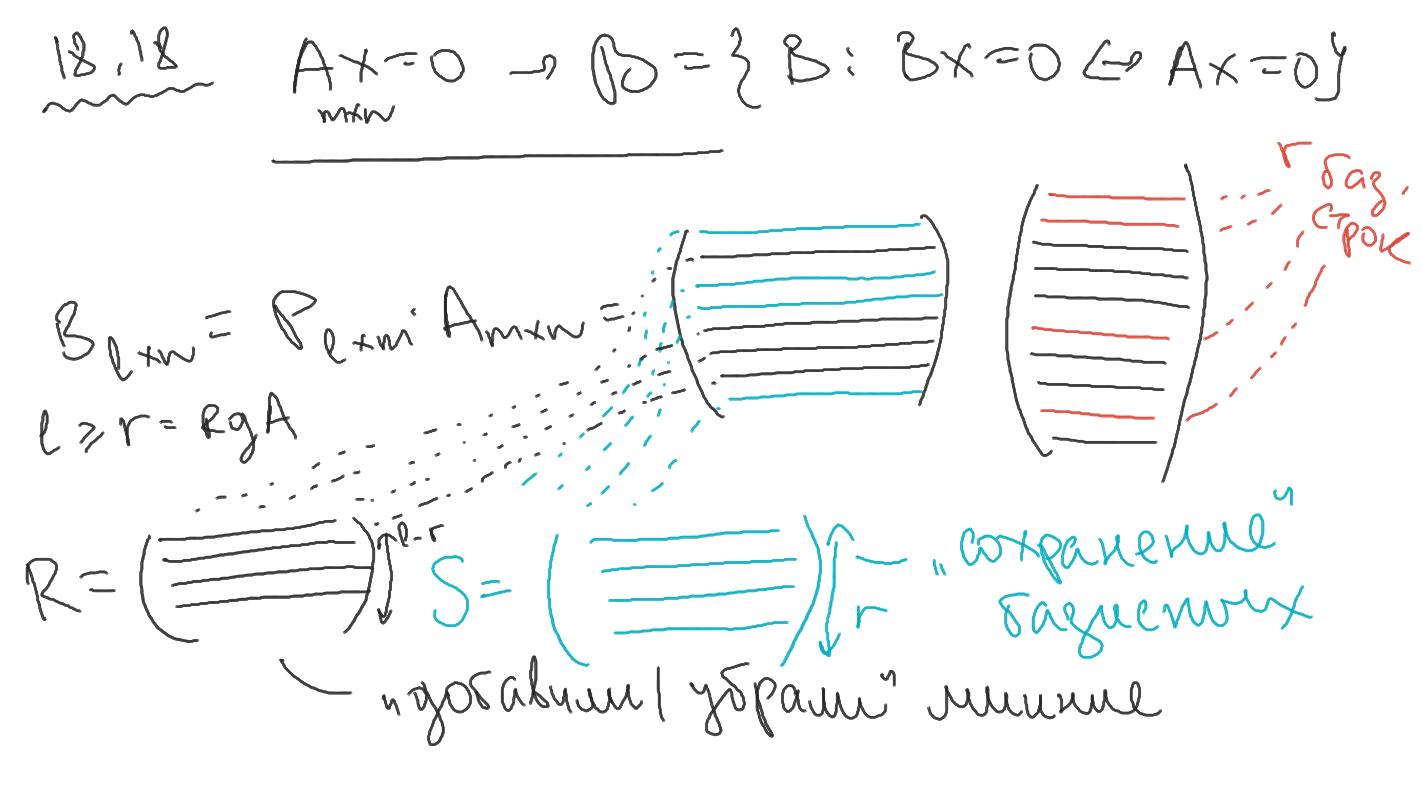
\includegraphics[width=0.8\columnwidth]{18.18.png}
    
      \caption{Подходит любая матрица $B$ вида $B \hm= PA$, где строчный ранг $P$ такой же, как у $A$ (равный $r$).
      И подматрица $S$ матрицы $P$, расположенная в $r$ базисных строках~---~это матрица, которая преобразует $r$ базисных строк матрицы $A$.}
      \label{fig:colourful-rows}
    \end{figure}
    
    \paragraph{P.S.}
    В конце задачника ответ сформулирован немного по-другому.
    Видимо, там считали, что строки матрицы $A$ линейно независимы (хотя в условии задачи про это не сказано).
    Если же строки $A$ линейно зависимы, то среди столбцов $P$ могут быть хоть нулевые (например, столбец, который во всех строках $B$ зануляет строку $A$, являющуюся линейной комбинацией базисных).
  \end{solution}
\end{document}
